\chapter{教師あり学習}

\section{トレーニングセットと仮説関数}

教師あり学習は,特徴量と目的変数の組のデータを用いて学習する.学習に使用するデータをトレーニングセットという.

\begin{defi}[トレーニングセット]
$\{(\bm{x}^{(i)},y^{(i)})\}_{i=1}^m \subset (({\cal X}_1 \times {\cal X}_2\times \cdots \times{\cal X}_n) \times {\cal Y})^m$を{\bf トレーニングセット(training set)}という.ここで,$m$は{\bf トレーニングサンプル数(number of training examples)},${\bm x}^{(i)} \in {\cal X}_1 \times {\cal X}_2\times \cdots \times {\cal X}_n$は$i$番目の$n$個の{\bf 入力変数(input variables)}または{\bf 特徴量(features)}で,${\bm x}^{(i)}=(x_1^{(i)},x_2^{(i)},\ldots,x_n^{(i)})^T$と表す.また,$y^{(i)} \in {\cal Y}$は$i$番目の{\bf 出力変数(output variable)}または{\bf 目的変数(target variable)}である.また,トレーニングセットの$i$番目の要素$({\bm x}^{(i)},y^{(i)})\in ({\cal X}_1 \times {\cal X}_2\times \cdots \times{\cal X}_n) \times {\cal Y}$を{\bf トレーニングサンプル(training example)}という.また,入力変数のとる空間${\cal X}_1 \times {\cal X}_2\times \cdots \times{\cal X}_n$を{\bf 入力変数空間(space of input values)},出力変数のとる空間${\cal Y}$を{\bf 出力変数空間(space of output values)}という.
\end{defi}

\begin{qu}
次のトレーニングセットにおいて,$x_3^{(4)},y^{(2)}$を答えよ.
\begin{table}[H]
\centering
\begin{tabular}{rrrrrr}
\hline
$i$ &$x_1^{(i)}$ &$x_2^{(i)}$ &$x_3^{(i)}$ &$x_4^{(i)}$ & $y^{(i)}$ \\ \hline
1 & 2104 & 5 & 1 & 45 & 460 \\
2 & 1416 & 3 & 2 & 40 & 232 \\
3 & 1534 & 3 & 2 & 30 & 315 \\
4 & 852  & 2 & 1 & 36 & 178 \\ \hline
\end{tabular}
\end{table}
\end{qu}
\begin{ans}
$x_3^{(4)}=1,~y^{(2)}=232$.\qed
\end{ans}

教師あり学習を使って解きたいタスク$T$は,入力変数から出力変数を予測することであるが,それは言い換えると入力変数を引数として出力変数を出力する写像を設定することである.この写像を仮説関数という.仮説関数を以下で定義する.

\begin{defi}[仮説関数]
入力変数${\bm x}$から出力変数$y$への写像$h:{\cal X}_1 \times {\cal X}_2\times \cdots \times{\cal X}_n \to {\cal Y}$,すなわち$h_{\bm \theta}({\bm x})$を{\bf 仮説関数(hypothesis function)}という.ここで,${\bm \theta}$は仮説関数の{\bf パラメータ}である(パラメータは複数あることがほとんどなのでベクトルとしている).
\end{defi}

すなわち,教師あり学習とは,仮説関数を設定し,トレーニングセットを用いて仮説関数の最適なパラメータを決定することといえる.最適なパラメータを決定できれば,そのパラメータをセットした仮説関数にデータを流し込むことで,そのデータに対する予測値を計算できる.

\section{線形回帰}

仮説関数は自らで与える必要があるが,仮説関数の形によって,教師あり学習に特別な名前がつくものがある.例えば,仮説関数を線形関数とし,出力変数空間を${\cal Y}=\mathbb{R}$としたときは線形回帰という.

\begin{defi}[線形回帰]
トレーニングセット$\{({\bm x}^{(i)},y^{(i)})\}_{i=1}^m \subset (({\cal X}_1 \times {\cal X}_2\times \cdots \times{\cal X}_n) \times {\cal Y})^m$について,${\cal Y}=\mathbb{R}$であり,かつ仮説関数が式(\ref{LM})である教師あり学習を,特に{\bf 線形回帰(linear regression)}という.ここで,特徴量${\bm x}^{(i)}$は,常に1の値をとるような特徴量$x_0^{(i)}=1$を付して${\bm x}^{(i)}=(x_0^{(i)},x_1^{(i)},x_2^{(i)},\ldots,x_n^{(i)})^T \in 1 \times {\cal X}_1 \times {\cal X}_2\times \cdots \times{\cal X}_n$と置き直すこととする.また,${\bm \theta}=(\theta_0,\theta_1,\ldots,\theta_n)^T \in \mathbb{R}^{n+1}$とする.
\begin{align}
h_{{\bm \theta}}({\bm x}^{(i)}) &= \theta_0 x_0^{(i)}+\theta_1 x_1^{(i)} +\theta_2 x_2^{(i)}+\cdots + \theta_n x_n^{(i)} \nonumber \\
&= \sum_{j=0}^n \theta_j x_j^{(i)}\nonumber \\
&= {\bm \theta}^T {\bm x}^{(i)} \label{LM}
\end{align}
\end{defi}

\begin{qu}
ある大学生について,1年次の成績で優をとった個数から2年次にいくつ優をとるのか予測したい.そこで,何人かの大学生の1年次の成績の優の個数$x$と2年次の成績の優の個数$y$を集めた.その結果が次表である.このとき,次の問いに答えよ.
\begin{table}[H]
\centering
\begin{tabular}{rr}
\hline
$x$    & $y$   \\ \hline
3 & 4 \\
2 & 1 \\
4 & 3 \\
0  & 1 \\ \hline
\end{tabular}
\end{table}
\begin{enumerate}
\item $m$はいくつか.
\item 仮説関数として$h_{{\bm \theta}}(x)=\theta_0+\theta_1 x$を設定し,本トレーニングセットを用いて線形回帰を行なった結果,パラメータは$\theta_0=-1,~\theta_1=2$となった.このとき,1年次の優の個数が6だった大学生の2年次の優の個数を予測せよ.
\end{enumerate}
\end{qu}
\begin{ans} 
\begin{enumerate}
\item $m=4$.
\item $h_{{\bm \theta}}(x)=-1+2x$なので,$h_{{\bm \theta}}(6)=-1+2\cdot 6=11$.
\end{enumerate}
\qed	
\end{ans}

\subsection{目的関数}

さて,仮説関数のパラメータをどう決めるかという問題がある.パラメータをでたらめに与えても良い予測値を返さないので,経験$E$のトレーニングセットを使って,性能指標$P$を高めるように仮説関数のパラメータをアップデートしていくことが必要になる.この手順を学習アルゴリズムといい,性能指標を測る関数を目的関数という.

\begin{defi}[学習アルゴリズム,目的関数]
性能指標を測る関数$J({\bm \theta})$を{\bf 目的関数}または{\bf コスト関数(cost function)}といい,この目的関数で測った性能指標が良くなるように仮説関数(のパラメータ${\bm \theta}$)をアップデートしていく手順を{\bf 学習アルゴリズム(learning algorithm)}という.
\end{defi}

回帰問題における性能指標としては,各トレーニングサンプル$({\bm x}^{(i)},y^{(i)})$での仮説関数$h_{{\bm \theta}}({\bm x}^{(i)})$と$y^{(i)}$の二乗誤差平均が考えられる.この二乗誤差平均を計算する目的関数を最小二乗誤差関数という.

\begin{defi}[最小二乗誤差関数]
トレーニングセット$\{({\bm x}^{(i)},y^{(i)})\}_{i=1}^m \subset ((1 \times {\cal X}_1 \times {\cal X}_2\times \cdots \times{\cal X}_n) \times {\cal Y})^m$について,式(\ref{SEF})で表される目的関数$J({\bm \theta})$を{\bf 最小二乗誤差関数(squared error function)}という.
\begin{align}
J({\bm \theta}) = \frac{1}{2m}\sum_{i=1}^m (h_{{\bm \theta}}({\bm x}^{(i)})-y^{(i)})^2 \label{SEF}
\end{align}
\end{defi}

\begin{rem}
$m$ではなく$2m$で割っているのは,微分したときに出てくる2が消えるようにしているからである.$m$でも特段の問題はない(同じ結果が得られる).
\end{rem}

\begin{qu}
あるトレーニングセット$\{(x^{(i)},y^{(i)})\}_{i=1}^3$をプロットしたところ以下の散布図となった(簡単のため,特徴量$x$に$x_0=1$である特徴量は追加していない).仮説関数を$h_{\theta}(x)=\theta x$,目的関数$J(\theta)$を最小二乗誤差関数としたとき,$J(0)$を求めよ.
\vspace{-10pt}
\begin{figure}[H]
\begin{center}
\includegraphics[width=8.0cm]{code/lrfig1.eps}
\vspace{-10pt}
\caption{\texttt{lrfig1.eps}}
\end{center}
\end{figure}
\vspace{-25pt}
\end{qu}
\begin{ans}
目的関数$J(\theta)$は次式となる.
\begin{align*}
J(\theta)&=\frac{1}{6}\sum_{i=1}^3 (h_{\theta}(x^{(i)})-y^{(i)})^2 \\
&=\frac{1}{6}\sum_{i=1}^3 (\theta x^{(i)}-y^{(i)})^2
\end{align*}
$\theta =0$を代入し,散布図から$y^{(i)}$を読み取ると,
\begin{align*}
J(0)&=\frac{1}{6}\sum_{i=1}^3 (-y^{(i)})^2 \\
&=\frac{1}{6}((-1)^2+(-2)^2+(-3)^2) \\
&= \frac{14}{6}
\end{align*}
\qed
\end{ans}

\begin{cod}[\texttt{lrfig1.eps}作成プログラム(\texttt{lrfig1.py})] 
\lstinputlisting[backgroundcolor={\color[gray]{.95}}]{code/lrfig1.py}
\end{cod}

\subsection{最急降下法}

「性能指標が良くなるように仮説関数のパラメータ${\bm \theta}$をアップデートしていく」とはどういうことか.目的関数が最小二乗誤差関数の場合,その最小二乗誤差がどんどん小さくなっていくことが,性能指標が良くなっていくといえる.すなわち,目的関数を最小にするパラメータ${\bm \theta}$を見つければよい.それを見つけるための手法が学習アルゴリズムである.

学習アルゴリズムの中で一般的なものとして最急降下法がある.最急降下法とは,目的関数$J({\bm \theta})$のグラフ上に適当に点を打ち(すなわちパラメータ${\bm \theta}$として適当に初期値を決め),その点からあたりを見渡してもっとも勾配が急な方向に一定程度進み,進んだ後の点からまたあたりを見渡してもっとも勾配が急な方向に一定程度進み\ldots を繰り返して,どこを見渡しても勾配がないような点を探す方法である.

最急降下法を行うためには,関数上のある点について勾配が急な方向はどの方向であるかを計算しなければならない.勾配が最も急な方向を向くベクトルを勾配ベクトルといい,以下で定義される.
\begin{defi}[勾配ベクトル]
$k$次元ベクトル${\bm \theta}=(\theta_1,\theta_2,\ldots,\theta_k)^T$からスカラー値に写る関数$f({\bm \theta})$,すなわち$f:{\bm \theta} \in \mathbb{R}^k \to \mathbb{R}$である関数$f({\bm \theta})$において,{\bf 勾配ベクトル}$\nabla_{{\bm \theta}}f=\frac{\partial f}{\partial {\bm \theta}}$は次式で定義される.
\begin{align}
\nabla_{{\bm \theta}}f = \frac{\partial f}{\partial {\bm \theta}} = 
\begin{bmatrix}
\frac{\partial f}{\partial \theta_1} \\[5pt]
\frac{\partial f}{\partial \theta_2} \\[3pt]
\vdots \\[5pt]
\frac{\partial f}{\partial \theta_k}
\end{bmatrix}
\end{align}
\end{defi}

\begin{qu}
$f:\mathbb{R}^2 \to \mathbb{R}$の関数$f(x,y)$のある点P$(x,y)$における最大勾配方向が勾配ベクトルの方向と同方向であることを示せ.
\end{qu}
\begin{ans}
勾配とは,関数$f$の変化度合いであり,勾配が最大ということは,関数の変化度合いが最も大きいということである.点P$(x,y)$と,そこから微小量$\Delta x$,$\Delta y$だけ動かした点Q$(x+\Delta x,y+\Delta y)$においてそれぞれ関数値を求めて差をとったものを変化度合い$\Delta f$とすると,$\overrightarrow{PQ}=\overrightarrow{OQ}-\overrightarrow{OP}=(\Delta x,\Delta y)$に注意して,以下の通り変形できる.
\begin{align*}
\Delta f &= f(x+\Delta x,y+\Delta y)-f(x,y) \\
&= f(x+\Delta x,y+\Delta y) -f(x,y+\Delta y)+f(x,y+\Delta y) -f(x,y) \\
&= \frac{f(x+\Delta x,y+\Delta y) -f(x,y+\Delta y)}{\Delta x}\Delta x +\frac{f(x,y+\Delta y) -f(x,y)}{\Delta y}\Delta y \\
&\fallingdotseq \frac{\partial f}{\partial x}\Delta x +\frac{\partial f}{\partial y}\Delta y \\
&= \nabla f \cdot (\Delta x,\Delta y) \\
&= \nabla f \cdot \overrightarrow{PQ}
\end{align*}
すなわちこれは,関数の変化度合いは勾配ベクトルと点Pから点Qへの方向ベクトル,すなわち微小量を動かした方向のベクトルの内積となっている.ここで,角度の定義より,
\begin{align*}
\Delta f &= ||\nabla f||||\overrightarrow{PQ}||\cos \theta
\end{align*}
となる.ここで,$\theta$は,$\nabla f$と$\overrightarrow{PQ}$のなす角である.関数の変化度合い$\Delta f$が最大となるのは,$\cos \theta =1$,すなわち$\theta =0$となる場合である.これはつまり$\nabla f$と$\overrightarrow{PQ}$が同じ方向を向いているときに関数の変化度合い$\Delta f$が最大となるということである.以上より,点Pから関数の変化度合い$\Delta f$が最大となるように進むためには(点Qをとるためには),勾配ベクトルの方向に進めばよいということである.\qed
\end{ans}

これで勾配が最も急な方向が勾配ベクトル方向であることがわかったので,それを用いて最急降下法を以下の通り定義する.
\begin{defi}[最急降下法]
関数$J({\bm \theta})$を最小とする${\bm \theta}$を次の手順で見つけるアルゴリズムを,{\bf 最急降下法(gradient descent algorithm)}という.ここで,$\alpha (>0)$を{\bf 学習率}といい,勾配が最大の方向にどの程度移動させるかの強さを表す.
\begin{algorithm}[H]
\caption{最急降下法}
\begin{algorithmic}[1]
\State{トレーニングセット$\{({\bm x}^{(i)},y^{(i)})\}_{i=1}^m$,仮説関数$h_{\bm \theta}({\bm x})$,目的関数$J({\bm \theta)}$を用意}
\State{$\alpha \gets 初期値$}
\State{${\bm \theta} \gets 初期値$}
\While{${\bm \theta}$が収束または有限回繰り返し}
\State{$\{({\bm x}^{(i)},y^{(i)})\}_{i=1}^m$を代入して$J({\bm \theta)}$を計算}
\State{$\nabla_{{\bm \theta}}J$を計算}

\State{${\bm \theta} \gets {\bm \theta}-\alpha \nabla_{{\bm \theta}}J$}\Comment{パラメータ$\theta_0,\theta_1\ldots $は同タイミングで更新}
\EndWhile
\end{algorithmic}
\end{algorithm}
\end{defi}

\begin{qu}
$x_0^{(i)}=1$も含め特徴量が$n+1$個のトレーニングセット$\{({\bm x}^{(i)},y^{(i)})\}_{i=1}^m$の線形回帰において,目的関数$J({\bm \theta})$を最小二乗誤差関数としたとき,$\nabla_{{\bm \theta}}J$を計算せよ.
\end{qu}
\begin{ans}
$\nabla_{{\bm \theta}}J$の$j$番目の要素$\frac{\partial J}{\partial \theta_j}$を計算すると以下となる.
\begin{align*}
\frac{\partial J}{\partial \theta_j}&= \frac{1}{2m}\sum_{i=1}^m \frac{\partial }{\partial \theta_j}(h_{{\bm \theta}}({\bm x}^{(i)})-y^{(i)})^2 \\
&=\frac{1}{2m}\sum_{i=1}^m 2(h_{{\bm \theta}}({\bm x}^{(i)})-y^{(i)})\frac{\partial }{\partial \theta_j}h_{{\bm \theta}}({\bm x}^{(i)})\\
&= \frac{1}{m}\sum_{i=1}^m (h_{{\bm \theta}}({\bm x}^{(i)})-y^{(i)})x_j^{(i)}
\end{align*}
$j=0$のときは$\frac{\partial }{\partial \theta_0}h_{{\bm \theta}}({\bm x}^{(i)})=1$であることに注意してまとめると,
\begin{align}
\nabla_{{\bm \theta}}J =\frac{1}{m}
\begin{bmatrix}
\sum_{i=1}^m (h_{{\bm \theta}}({\bm x}^{(i)})-y^{(i)}) \\[3pt]
\sum_{i=1}^m (h_{{\bm \theta}}({\bm x}^{(i)})-y^{(i)})x_1^{(i)} \\[3pt]
\sum_{i=1}^m (h_{{\bm \theta}}({\bm x}^{(i)})-y^{(i)})x_2^{(i)} \\[3pt]
\vdots \\[3pt]
\sum_{i=1}^m (h_{{\bm \theta}}({\bm x}^{(i)})-y^{(i)})x_j^{(i)} \\[3pt]
\vdots \\[3pt]
\sum_{i=1}^m (h_{{\bm \theta}}({\bm x}^{(i)})-y^{(i)})x_n^{(i)} \\[3pt]
\end{bmatrix}\label{simpleJ}
\end{align}
となる($\nabla_{{\bm \theta}}J$は$n+1$次元ベクトルである).\qed
\end{ans}

\subsection{デザイン行列}

最急降下法アルゴリズムは, 式(\ref{simpleJ})を用いて$\nabla_{{\bm \theta}}J$の各要素に対して逐次計算を行っていけば単純に実装できるが,各要素の和の計算を各要素に対して行い,反復していくことは少々ややこしい.行列計算を容易に行えるプログラミング言語で実装する場合には,できるだけ逐次計算をしないように,行列計算やベクトル計算を用いて工夫して実装することが簡潔かつバグも少ない.ここでは,デザイン行列を定義し,行列計算により$\nabla_{{\bm \theta}}J$を計算できることを示す.

\begin{defi}[デザイン行列]
$x_0^{(i)}=1$も含め特徴量が$n+1$個のトレーニングセット$\{({\bm x}^{(i)},y^{(i)})\}_{i=1}^m$において,式(\ref{designX})で定義する行列$X \in \mathbb{R}^{m\times (n+1)}$を{\bf デザイン行列(design matrix)}という.デザイン行列は,特徴量${\bm x}^{(i)}$を転置してサンプル数の分縦に並べたもので表される.ここで,特徴量として$x_0=1$が加わっていることに注意する.
\begin{align}
X = 
\begin{bmatrix}
\mbox{------} & {{\bm x}^{(1)}}^T & \mbox{------} \\
\mbox{------} & {{\bm x}^{(2)}}^T & \mbox{------} \\
 & \vdots & \\
\mbox{------} & {{\bm x}^{(m)}}^T & \mbox{------}
\end{bmatrix}
=
\begin{bmatrix}
1 & x_1^{(1)} & x_2^{(1)} & \cdots & x_n^{(1)} \\
1 & x_1^{(2)} & x_2^{(2)} & \cdots & x_n^{(2)} \\
\vdots & \vdots & \vdots & \vdots & \vdots \\
1 & x_1^{(m)} & x_2^{(m)} & \cdots & x_n^{(m)} 
\end{bmatrix} \label{designX}
\end{align}
\end{defi}

\begin{qu}
次のトレーニングセットにおいて,デザイン行列$X$を答えよ.
\begin{table}[H]
\centering
\begin{tabular}{cccccc}
\hline
$i$ &$x_1^{(i)}$ &$x_2^{(i)}$ &$x_3^{(i)}$ &$x_4^{(i)}$ & $y^{(i)}$ \\ \hline
1 & 2104 & 5 & 1 & 45 & 460 \\
2 & 1416 & 3 & 2 & 40 & 232 \\
3 & 1534 & 3 & 2 & 30 & 315 \\
4 & 852  & 2 & 1 & 36 & 178 \\ \hline
\end{tabular}
\end{table}
\end{qu}
\begin{ans}
サンプル数が4つで,特徴量が$x_0=1$を含めると5つなので,$X$は$4\times 5$次元の行列となり,
\begin{align*}
X=
\begin{bmatrix}
1 & 2104 & 5 & 1 & 45 \\
1 & 1416 & 3 & 2 & 40 \\
1 & 1534 & 3 & 2 & 30 \\
1 & 852  & 2 & 1 & 36 
\end{bmatrix}
\end{align*}\qed
\end{ans}

デザイン行列を使うと,予測値である線形回帰の仮説関数のベクトルを簡潔に表すことができ,1発の線形代数計算で予測値を計算できる.

\begin{qu}
$x_0^{(i)}=1$も含め特徴量が$n+1$個のトレーニングセット$\{({\bm x}^{(i)},y^{(i)})\}_{i=1}^m$における線形回帰問題を考える.このとき,$(h_{{\bm \theta}}({\bm x}^{(1)}),h_{{\bm \theta}}({\bm x}^{(2)}),\ldots,h_{{\bm \theta}}({\bm x}^{(m)}))^T$を$X$,${\bm \theta}$を用いて表せ.
\end{qu}
\begin{ans}
式(\ref{tenkai1})より,以下となる.
\begin{align}
\begin{bmatrix}
h_{{\bm \theta}}({\bm x}^{(1)}) \\
h_{{\bm \theta}}({\bm x}^{(2)}) \\
\vdots \\
h_{{\bm \theta}}({\bm x}^{(m)})
\end{bmatrix}
=
\begin{bmatrix}
{\bm \theta}^T{\bm x}^{(1)} \\
{\bm \theta}^T {\bm x}^{(2)}\\
\vdots \\
{\bm \theta}^T {\bm x}^{(m)}
\end{bmatrix}
=
\begin{bmatrix}
{{\bm x}^{(1)}}^T{\bm \theta} \\
{{\bm x}^{(2)}}^T{\bm \theta} \\
\vdots \\
{{\bm x}^{(m)}}^T{\bm \theta}
\end{bmatrix}
=
\begin{bmatrix}
\mbox{------} & {{\bm x}^{(1)}}^T & \mbox{------} \\
\mbox{------} & {{\bm x}^{(2)}}^T & \mbox{------} \\
 & \vdots & \\
\mbox{------} & {{\bm x}^{(m)}}^T & \mbox{------}
\end{bmatrix}
\begin{bmatrix}
| \\[-2pt]
| \\
{\bm \theta} \\
| \\[-2pt]
|
\end{bmatrix}
=X {\bm \theta} \label{lr_hypo}
\end{align}
\qed
\end{ans}

この結果を用いることで,目的関数を最小二乗誤差関数とした線形回帰問題において,目的関数をより簡潔に表すことができる.

\begin{qu}
$x_0^{(i)}=1$も含め特徴量が$n+1$個のトレーニングセット$\{({\bm x}^{(i)},y^{(i)})\}_{i=1}^m$における線形回帰問題において,目的関数$J({\bm \theta})$を最小二乗誤差関数とする.このとき,$J({\bm \theta})$を$X$,${\bm \theta}$,${\bm y}$を用いて表せ.ここで,${\bm y}=(y^{(1)},y^{(2)},\ldots,y^{(m)})^T$とする.
\end{qu}
\begin{ans}
\begin{align}
J({\bm \theta})&= \frac{1}{2m}\sum_{i=1}^m (h_{{\bm \theta}}({\bm x}^{(i)})-y^{(i)})^2 \nonumber \\
&=\frac{1}{2m}
\begin{bmatrix}
h_{{\bm \theta}}({\bm x}^{(1)})-y^{(1)} & h_{{\bm \theta}}({\bm x}^{(2)})-y^{(2)} & \cdots & h_{{\bm \theta}}({\bm x}^{(m)})-y^{(m)}
\end{bmatrix}
\begin{bmatrix}
h_{{\bm \theta}}({\bm x}^{(1)})-y^{(1)} \\
h_{{\bm \theta}}({\bm x}^{(2)})-y^{(2)} \\
\vdots \\
h_{{\bm \theta}}({\bm x}^{(m)})-y^{(m)}
\end{bmatrix}\nonumber
\end{align}
となるが,ここで,
\begin{align}
\begin{bmatrix}
h_{{\bm \theta}}({\bm x}^{(1)})-y^{(1)} \\
h_{{\bm \theta}}({\bm x}^{(2)})-y^{(2)} \\
\vdots \\
h_{{\bm \theta}}({\bm x}^{(m)})-y^{(m)}
\end{bmatrix}
=
\begin{bmatrix}
h_{{\bm \theta}}({\bm x}^{(1)}) \\
h_{{\bm \theta}}({\bm x}^{(2)}) \\
\vdots \\
h_{{\bm \theta}}({\bm x}^{(m)})
\end{bmatrix}
-
\begin{bmatrix}
y^{(1)} \\
y^{(2)} \\
\vdots \\
y^{(m)}
\end{bmatrix}
=X{\bm \theta}-{\bm y} \nonumber
\end{align}
より,
\begin{align}
J({\bm \theta})&= \frac{1}{2m}(X{\bm \theta}-{\bm y})^T(X{\bm \theta}-{\bm y}) \label{lr_cost}
\end{align}\qed
\end{ans}

これで目的関数を簡潔に書けたので,最後にそれを微分して$\nabla_{{\bm \theta}}J$を求める.ここで,線形形式,二次形式の勾配ベクトルを使用するので事前に述べておく.
\begin{theo}[線形形式,二次形式の勾配ベクトル]
$n$次元列ベクトル${\bm x},{\bm a}$,$n\times n$行列$A$に対して,次式が成り立つ.
\begin{align}
\nabla_{{\bm x}}({\bm a}^T {\bm x})&=\nabla_{{\bm x}}({\bm x}^T {\bm a})={\bm a}\\
\nabla_{{\bm x}}({\bm x}^T A{\bm x})&=(A+A^T){\bm x}
\end{align}
\end{theo}
\begin{pro}
線形形式の勾配ベクトルの証明は略.二次形式の勾配ベクトルは式(\ref{quadform})から計算すると楽である.式(\ref{quadform})において,$x_i$における偏微分を計算すると以下となる.変形の最後は,$A=\{a_{ij}\}$の転置行列を$A^T=\{a'_{ij}\}$としたとき,$a_{ki}=a'_{ik}$であることを使用している.
\begin{align*}
\frac{\partial }{\partial x_i}({\bm x}^T A{\bm x})&=\frac{\partial }{\partial x_i}\left(a_{ii}x_i^2+\sum_{\substack{j=1\\j\neq i}}^n a_{ij}x_ix_j+\sum_{\substack{k=1\\k\neq i}}^n a_{ki}x_kx_i+\sum_{\substack{j,k\\j\neq i\\k\neq i}}a_{kj}x_kx_j\right) 	\\
&=2a_{ii}x_i+\sum_{\substack{j=1\\j\neq i}}^n a_{ij}x_j+\sum_{\substack{k=1\\k\neq i}}^n a_{ki}x_k\\
&=\sum_{j=1}^na_{ij}x_j+\sum_{k=1}^na_{ki}x_k\\
&=\sum_{j=1}^na_{ij}x_j+\sum_{k=1}^na'_{ik}x_k
\end{align*}
第1項について,$x_1〜x_n$についての結果を列ベクトルとして並べると,式(\ref{tenkai2})の形が現れ,その結果は$A{\bm x}$となる.第2項についても同様であり,その結果は$A^T{\bm x}$となる.以上より,$\nabla_{{\bm x}}({\bm x}^T A{\bm x})=A{\bm x}+A^T{\bm x}=(A+A^T){\bm x}$である.
\qed	
\end{pro}

\begin{qu}
$x_0^{(i)}=1$も含め特徴量が$n+1$個のトレーニングセット$\{({\bm x}^{(i)},y^{(i)})\}_{i=1}^m$における線形回帰問題において,目的関数$J({\bm \theta})$を最小二乗誤差関数とする.このとき,$\nabla_{{\bm \theta}}J$を$m$,$X$,${\bm \theta}$,${\bm y}$で表せ.
\end{qu}
\begin{ans}
$X^TX$は対称行列であることに注意すると,
\begin{align}
\nabla_{{\bm \theta}}J&=\nabla_{{\bm \theta}}\left(\frac{1}{2m}(X{\bm \theta}-{\bm y})^T(X{\bm \theta}-{\bm y})\right) \nonumber\\
&=\nabla_{{\bm \theta}}\left(\frac{1}{2m}\left((X{\bm \theta})^T(X{\bm \theta})-(X{\bm \theta})^T{\bm y}-{\bm y}^T(X{\bm \theta})+{\bm y}^T{\bm y}\right)\right)\nonumber\\
&=\nabla_{{\bm \theta}}\left(\frac{1}{2m}\left((X{\bm \theta})^T(X{\bm \theta})-2(X{\bm \theta})^T{\bm y}+{\bm y}^T{\bm y}\right)\right)\nonumber\\
&=\nabla_{{\bm \theta}}\left(\frac{1}{2m}\left( {\bm \theta}^TX^TX{\bm \theta}-2{\bm \theta}^TX^T{\bm y}+{\bm y}^T{\bm y} \right)\right) \nonumber\\
&=\frac{1}{2m}\left(\nabla_{{\bm \theta}}({\bm \theta}^TX^TX{\bm \theta})-2\nabla_{{\bm \theta}}({\bm \theta}^TX^T{\bm y})+\nabla_{{\bm \theta}}({\bm y}^T{\bm y})\right)\nonumber\\
&=\frac{1}{2m}\left(2X^TX{\bm \theta}-2X^T{\bm y}\right)\nonumber \\
&=\frac{1}{m}\left(X^TX{\bm \theta}-X^T{\bm y}\right) \label{LRglad}
\end{align}\qed
\end{ans}

\subsection{Pythonによる実装}

以上で線形回帰で必要なパーツは揃った.これらのパーツを実際にPythonにて実装していきながら,線形回帰とはどういうものかを掴んでいく.

\begin{qu}\label{qu_lr5}
\texttt{ex1data1.txt}(2列,カンマ区切り,列名ヘッダーなし,1列目はpopulation of city in 10,000s,2列目はprofit in \$10,000sであるデータ)を散布図でプロットせよ.
\end{qu}
\begin{ans}
\begin{cod}[\texttt{lr5.py}] 
\lstinputlisting[backgroundcolor={\color[gray]{.95}}]{code/lr5.py}
\vspace{-19pt}
\begin{figure}[H]
\begin{center}
\framed
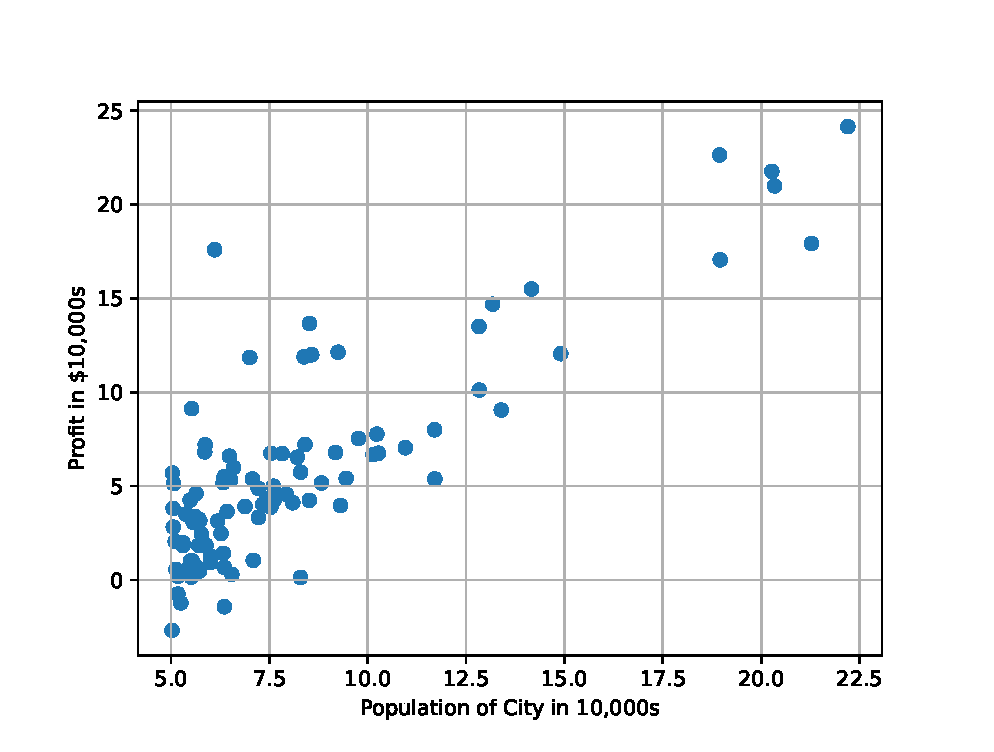
\includegraphics[width=8.0cm]{code/lrfig2.eps}
\vspace{-10pt}
\caption{\texttt{lrfig2.eps}}
\endframed
\end{center}
\end{figure}
%\begin{lstlisting}
%\end{lstlisting}
\end{cod}
\vspace{-20pt}
\end{ans}


\begin{qu}\label{qu_lr1}
(問題\ref{qu_lr5}の続き) \texttt{ex1data1.txt}から,デザイン行列$X$と目的変数${\bm y}$をそれぞれ\texttt{<2d\_ndarray>}で作成せよ.ここで,目的変数はprofit in \$10,000sとし,デザイン行列には$x_0^{(i)}=1$の項も付け加えよ.
\end{qu}
\begin{ans}
表形式データは,行方向にデータが並び,列方向が特徴量が並ぶものが多いので,デザイン行列は表形式データそのものとして与えてあげればよい.また,目的変数は1列のデータであるが,\texttt{<DataFrame>}から1列だけ読み込む場合は\texttt{<1d\_ndarray>}になってしまうので,列ベクトルとしての\texttt{<2d\_ndarray>}に変換する.なお,データ数が多いので,以下のコードにおいてはデザイン行列や目的変数は最初の5行分のみ表示するようにしている.
\begin{cod}[\texttt{lr1.py}] 
\lstinputlisting[backgroundcolor={\color[gray]{.95}}]{code/lr1.py}
\vspace{-10pt}
\begin{lstlisting}
X=
[[1.     6.1101]
 [1.     5.5277]
 [1.     8.5186]
 [1.     7.0032]
 [1.     5.8598]]
......
type=<class 'numpy.ndarray'>,shape=(97, 2)
y=
[[17.592 ]
 [ 9.1302]
 [13.662 ]
 [11.854 ]
 [ 6.8233]]
......
type=<class 'numpy.ndarray'>,shape=(97, 1)
\end{lstlisting}
\end{cod}
\vspace{-10pt}
\qed
\end{ans}

\begin{qu}\label{qu_lr2}
(問題\ref{qu_lr1}の続き) 仮説関数のパラメータを$\bm{\theta}=(1,-2)^T$とする.このとき,問題\ref{qu_lr1}で作成したデザイン行列$X$に対して予測値である仮説関数ベクトル$(h_{{\bm \theta}}({\bm x}^{(1)}),h_{{\bm \theta}}({\bm x}^{(2)}),\ldots,h_{{\bm \theta}}({\bm x}^{(m)}))^T$を計算し,問題\ref{qu_lr1}で作成した目的変数${\bm y}$と並べて表示せよ.なお,仮説関数は関数として定義せよ.
\end{qu}
\begin{ans}
式(\ref{lr_hypo})を実装すれば良い.
\begin{cod}[\texttt{lr2.py}] 
\lstinputlisting[backgroundcolor={\color[gray]{.95}}]{code/lr2.py}
\vspace{-10pt}
\begin{lstlisting}
y_df=
         y   y_pred
0  17.5920 -11.2202
1   9.1302 -10.0554
2  13.6620 -16.0372
3  11.8540 -13.0064
4   6.8233 -10.7196
\end{lstlisting}
\end{cod}
\vspace{-10pt}
予測結果より,$\bm{\theta}=(1,-2)^T$では全然予測になっていないことがわかる.
\qed
\end{ans}

\begin{qu}\label{qu_lr3}
(問題\ref{qu_lr2}の続き) 仮説関数のパラメータを$\bm{\theta}=(1,-2)^T$とする.このとき,問題\ref{qu_lr1}で作成したデザイン行列$X$と目的変数${\bm y}$に対して目的関数$J({\bm \theta})$の値を計算せよ.なお,目的関数$J({\bm \theta})$は関数として定義せよ.
\end{qu}
\begin{ans}
式(\ref{lr_cost})を実装すれば良い.numpyでの線形代数計算は,結果がスカラーだとしても\texttt{<2d\_ndarray>}のままなので,要素を指定してあげて数値を取り出すことが必要となる.
\begin{cod}[\texttt{lr3.py}] 
\lstinputlisting[backgroundcolor={\color[gray]{.95}}]{code/lr3.py}
\vspace{-10pt}
\begin{lstlisting}
J=303.8795839611464
\end{lstlisting}
\end{cod}
\vspace{-10pt}
目的関数の数値の大きさからも,${\bm \theta}$は最適化できていないことがわかる.
\qed
\end{ans}

\begin{qu}\label{qu_lr6}
(問題\ref{qu_lr3}の続き) 仮説関数のパラメータを$\bm{\theta}=(1,-2)^T$とする.このとき,問題\ref{qu_lr2}で計算した予測値を線でプロットせよ.
\end{qu}
\begin{ans}
\begin{cod}[\texttt{lr6.py}] 
\lstinputlisting[backgroundcolor={\color[gray]{.95}}]{code/lr6.py}
\vspace{-19pt}
\begin{figure}[H]
\begin{center}
\framed
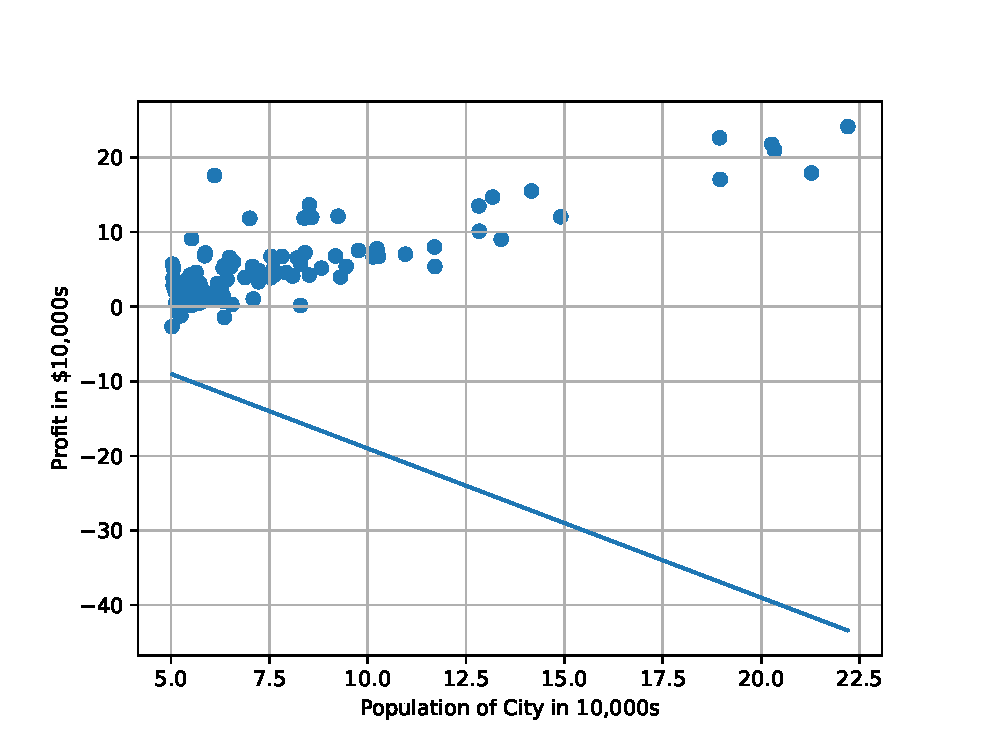
\includegraphics[width=8.0cm]{code/lrfig3.eps}
\vspace{-10pt}
\caption{\texttt{lrfig3.eps}}
\endframed
\end{center}
\end{figure}
%\begin{lstlisting}
%\end{lstlisting}
\end{cod}
\vspace{-20pt}
図示すると予測が全然できていないことが一目瞭然.
\qed	
\end{ans}



\begin{qu}\label{qu_lr4}
(問題\ref{qu_lr6}の続き) \texttt{ex1data1.txt}のデータを全て用いて目的変数${\bm y}$を特徴量から予測するモデルを線形回帰で構築するとしたとき,次の問いに答えよ.
\begin{enumerate}
\item 線形回帰の予測値である仮説関数$h_{{\bm \theta}}({\bm x})$のパラメータ${\bm \theta}$を求めよ.ここで,目的関数$J({\bm \theta})$は最小二乗誤差関数とし,${\bm \theta}$を求めるときに使用するアルゴリズムは最急降下法とする.また,最急降下法の学習率$\alpha $は$\alpha = 0.01$,${\bm \theta}$の初期値は${\bm \theta}=(1,-2)^T$とし,収束判定は行わず1500回パラメータの更新を行ったらアルゴリズムは終了するように実装せよ.
\item 求めた${\bm \theta}$に対する目的関数$J({\bm \theta})$の値を求めよ.
\item 新しくpopulation of city in 10,000sのデータ$x=7.532$を得たとする.この$x$に対してprofit in \$10,000sがいくらになるか,上で構築した線形回帰モデルを用いて予測せよ.
\end{enumerate}
\end{qu}
\begin{ans}
最急降下法における$J({\bm \theta})$の勾配ベクトルは式(\ref{LRglad})を実装すればよい.その他,仮説関数や目的関数は問題\ref{qu_lr2},問題\ref{qu_lr3}で実装したものをベースに組めばよい.
\begin{cod}[\texttt{lr4.py}] 
\lstinputlisting[backgroundcolor={\color[gray]{.95}}]{code/lr4.py}
\vspace{-10pt}
\begin{lstlisting}
1: theta=
[[-3.55089376]
 [ 1.15838599]]
2: J=4.4878002526614615
3: y_pred=5.174069533566031
\end{lstlisting}
\end{cod}
\vspace{-10pt}
${\bm \theta}=(1,-2)^T$の場合の$J({\bm \theta})$の値からかなり減少していることがわかる.
\qed
\end{ans}







\subsection{デバッグ}

最急降下法がうまく収束しているかを確認する手段としては,ループ1回ごとに$J({\bm \theta})$の値をプロットしていき,値が順調に減少していっているかどうかをみるという方法がある.これをデバッグという.

\begin{defi}[デバッグ]
 \\
最急降下法において,横軸に繰り返し回数(number of iterations),縦軸に目的関数値$J({\bm \theta})$をとり図示することを{\bf デバッグ(debugging)}という.
\end{defi}

\subsection{正規方程式}

さて,最急降下法で収束して得られた${\bm \theta}$は,どこを見渡しても勾配がない状態となっている.これは,言い換えると目的関数$J({\bm \theta})$の勾配ベクトルがゼロベクトルとなる点${\bm \theta}$は,方程式$\nabla_{{\bm \theta}}J={\bm 0}$の解である.この方程式は正規方程式という.
\begin{defi}[正規方程式]
 \\
目的関数$J({\bm \theta})$の回帰問題について,次式を{\bf 正規方程式(normal equation formula)}という.
\begin{align}
\nabla_{{\bm \theta}}J={\bm 0}
\end{align}
\end{defi}

\begin{qu}
特徴量が$n$であるトレーニングセット$\{({\bm x}^{(i)},y^{(i)})\}_{i=1}^m$における線形回帰問題において,目的関数$J({\bm \theta})$を最小二乗誤差関数とする.このとき,$\nabla_{{\bm \theta}}J={\bm 0}$を簡単に表せ.
\end{qu}
\begin{ans}
式(\ref{LRglad})より,
\begin{align}
X^TX{\bm \theta}=X^T{\bm y}	
\end{align}\qed
\end{ans}
これを${\bm \theta}$について解けば最適なパラメータ${\bm \theta}$を得ることができる.ここで,$X^TX$が正則であれば,逆行列$(X^TX)^{-1}$が存在するのでそれを左から掛けることによって解けるが,正則でない場合(非正則,非可逆,特異の場合ともいう),逆行列を持たず,正規方程式は解を持たない(不能)もしくは複数または無数の解(不定)となる.不能や不定だからそれでお手上げ,というわけにはいかないので,「いい感じの」の解を設定したいとする.この「いい感じ」の解は,$X^TX$の{\bf ムーア・ペンローズ一般逆行列}$(X^TX)^+$を用いて,次式で書ける.
\begin{align}
{\bm \theta}=(X^TX)^+ X^T{\bm y}
\end{align}
この議論の詳細は,まだ著者が理解できていないため,今の所は割愛する.

では,どのような場合に$X^TX$は非正則なのか.ここは著者がまだ理解できていないが,\cite{AndrewML}によれば,以下2つの場合を念頭に置いておけばとりあえず良いとのこと.
\begin{enumerate}
\item {\bf 特徴量が冗長}:例えば,住宅価格の予測についての特徴量で,縦の長さ,横の長さ,面積の3つを考えた場合,面積は縦の長さと横の長さですでに捉えられているので,面積という特徴量が冗長である.
\item {\bf データ数より特徴量が多い}($m \leq n$):$n=100$個の特徴量を,$m=10$サンプルでフィッティングするのは,うまくいくこともあるかもしれないが良いアイデアではない.
\end{enumerate}


教師あり学習の回帰問題について,パラメータを探す方法として最急降下法と正規方程式を解く方法の2種類を取り上げた.それぞれの手法のメリットやデメリットについて,\cite{AndrewML}によれば以下の通り.
\begin{itemize}
\item 最急降下法は,学習率$\alpha $を適切に選択する必要があるため,良さげな数値を何度か試行することが必要となってくる場合がある.一方で,正規方程式はその手間がない.
\item 最急降下法の場合は,アルゴリズムがちゃんと機能しているか,ちゃんと収束しているかなどを確認しなければならないが,正規方程式はその手間がない.
\item 正規方程式の場合,特徴量スケーリングを行う必要はない.
\item 正規方程式は,逆行列を求める必要があるが,逆行列を計算するコストが非常に大きい.具体的には,逆行列の計算コストは特徴量$n$の3乗のオーダーとなる.一方,最急降下法は特徴量$n$本に対する計算を繰り返すだけなので,計算コストは$n$のオーダーと非常に少ない.つまり,最急降下法は特徴量が数百万個あるような場合でも正しく機能する.だいたい$n=10000$が正規方程式ではなく最急降下法を選ぶ目安.
\end{itemize}

\section{多項式回帰}

仮説関数として,線形関数を選ぶ必要はない.仮説関数として多項式を設定した場合は多項式回帰と呼ばれる.
\begin{defi}[多項式回帰]
 \\
回帰問題において,仮説関数を多項式とした場合,特に{\bf 多項式回帰(polynomial regression)}という.
\end{defi}

\begin{qu}
トレーニングセット$\{(x_1^{(i)},y^{(i)})\}_{i=1}^10$をプロットしたところ,下図となった.これについての回帰問題を解きたい.仮説関数としてどのようなものが考えられるか.

\end{qu}
\begin{proof}
新しく特徴量として$x_2^{(i)}=(x_1^{(i)})^2$を設定し,仮説関数として$h_{{\bm \theta}}(x^{(i)})=\theta_0+\theta_1 x_1^{(i)}+\theta_2 x_2^{(i)}=\theta_0+\theta_1 x_1^{(i)}+\theta_2 (x_1^{(i)})^2$とする.
\end{proof}

複数の特徴量がある場合,各特徴量のとりうる範囲がだいたい同じような範囲にあると,最急降下法の収束速度は速くなる.特徴量を変換してとりうる範囲の調整を行うことを,特徴量スケーリングという.

\begin{defi}[特徴量スケーリング]
 \\
トレーニングセット$\{({\bm x}^{(i)},y^{(i)})\}_{i=1}^m$について,${\bm x}^{(i)}$の各特徴量のとりうる範囲を同じような範囲に変換することを{\bf 特徴量スケーリング(feature scalling)}という.特に,特徴量$x_j$の平均$\mu_j$を用いて$\frac{x_j-\mu_j}{s_j}$のようにスケーリングすることを,{\bf 平均標準化(mean normalization)}という.ここで,$s_j$は,特徴量$x_j$の標準偏差または$\max - \min$とする.
\end{defi}
\begin{rem}
特徴量スケーリングの方法は何か定まった方法があるわけではない.例えば,最大値で割るとか,平均を引いて最大と最小の差で割るとか,なんとなく1000分の1するとか,やり方はなんでもよいし,特徴量ごとに異なる方法をとっても良い.大事なことは全ての特徴量をだいたい似たような範囲にもっていくことである.なお,範囲としては,Andrew Ng曰く,各特徴量の取りうる範囲がだいだい$-3〜3$の中の範囲をとるのを目安にしているとのこと.
\end{rem}

特に,多項式回帰の場合は特徴量のオーダーが他の特徴量と比べて極端に異なることが多いため,特徴量スケーリングがほとんど必須となってくる.

\begin{qu}
住宅の平米数から住宅価格を予測する回帰問題を解くことを考える.集めたデータの平米数はおおむね1から1000フィートの範囲となっている.平米数と価格をプロットしたところ,以下の仮説関数があてはまりがよさそうと考えた.
\begin{align*}
h_{{\bm \theta}}(x^{(i)})=\theta_0+\theta_1 平米数^{(i)}+\theta_2 \sqrt{平米数^{(i)}}
\end{align*}
ここで,特徴量スケーリングをしてより適切に回帰問題を解くために,新しく仮説関数を
\begin{align*}
h_{{\bm \theta}}(x^{(i)})=\theta_0+\theta_1 x_1^{(i)}+\theta_2 x_2^{(i)}
\end{align*}
としたとき,$x_1^{(i)}$と$x_2^{(i)}$はそれぞれどのようにおくのがよいか.ここで,$\sqrt{1000}\fallingdotseq 32$とする.
\end{qu}
\begin{proof}
$x_1^{(i)}=\frac{平米数^{(i)}}{1000}$,$x_2^{(i)}=\frac{\sqrt{平米数^{(i)}}}{32}$.
\end{proof}

特徴量は,与えられたものをそのまま使う必要はなく,それらを組み合わせるなどして自分で新しく作っても良い.うまく特徴量を作り出して,より単純な仮説関数にするという選択肢もある.

\begin{qu}
今,手元に特徴量$x_1^{(i)}$:間口,$x_2^{(i)}$:奥行き,出力変数$y^{(i)}$:土地の価格がある.このとき,土地の価格を予測する問題を線形回帰で解くことを考えると,仮説関数としてまず$h_{{\bm \theta}}({\bm x}^{(i)})=\theta_0+\theta_1 x_1^{(i)}+\theta_2 x_2^{(i)}$が考えつくが,もっと簡単に仮説関数を定めるにはどうすれば良いか.
\end{qu}
\begin{proof}
新しい特徴量$x_3^{(i)}=x_1^{(i)}x_2^{(i)}$:面積を設定し,仮説関数として$h_{{\bm \theta}}(x^{(i)})=\theta_0+\theta_1 x_3^{(i)}$とする.
\end{proof}
